% file: push-button.tex
%
% Use:
%
% 	$ pdflatex -shell-escape architecture.tex
%
% to generate a png image.
%

\documentclass[10pt,tikz,border=10,convert={outfile=\jobname.png}]{standalone}
\usetikzlibrary{calc,positioning,arrows.meta,shadows,fadings,through}
  
%% TODO: move these color definitions to a separate tex file.
\definecolor{regular}{HTML}{444444}
\definecolor{hover}{HTML}{384839}
\definecolor{down}{HTML}{384729}

\begin{document}
  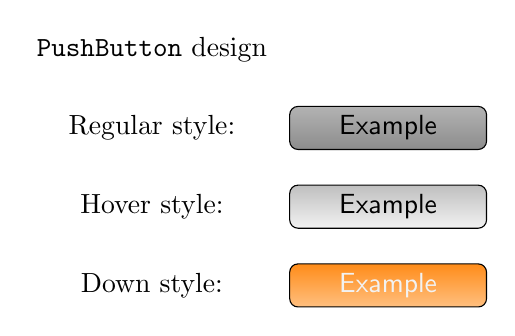
\begin{tikzpicture}[
    title/.style={},
    button/.style={rectangle,rounded corners=3pt,draw,minimum width=2.5cm}
  ]

    \node(title) [title] {{\ttfamily PushButton} design};
  
    \node(regular-title) [title,below of=title] {Regular style:};
    \node(regular-button) [button,right of=regular-title,xshift=2cm,shading = axis,left color=black!30!white,right color=black!45!white,shading angle=0] {\sffamily Example};

    \node(hover-title) [title,below of=regular-title] {Hover style:};
    \node(hover-button) [button,right of=hover-title,xshift=2cm,shading = axis,left color=black!5!white,right color=black!25!white,shading angle=180] {\sffamily Example};

    \node(down-title) [title,below of=hover-title] {Down style:};
    \node(down-button) [button,right of=down-title,xshift=2cm,shading = axis,left color=orange!50!white,right color=orange!90!white,shading angle=180,text=black!5!white] {\sffamily Example};

  \end{tikzpicture}

\end{document}
  